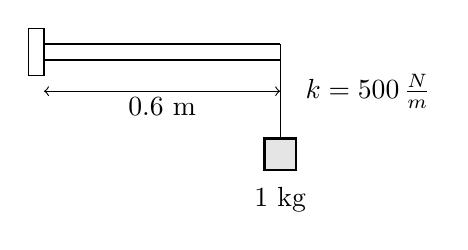
\begin{tikzpicture}
    % Draw the main beam
    \draw[thick] (0,0) -- (3,0);
    \draw[thick] (0,-0.2) -- (3,-0.2);
    
    % Add end support
    \draw (-0.2,-0.4) rectangle (0,0.2);
    
    % Add dimension line and label
    \draw[<->] (0,-0.6) -- (3,-0.6);
    \node at (1.5,-0.8) {0.6 m};
    
    % Draw spring
    \draw (3,0) -- (3, -1.2);
    \node[anchor=west] at (3.2, -0.6) {$k=500\,\frac{N}{m}$};
    
    % Draw mass
    \fill[gray!20] (2.8, -1.6) rectangle (3.2, -1.2);
    \draw[thick] (2.8, -1.6) rectangle (3.2, -1.2);
    \node[anchor=north] at (3, -1.7) {1 kg};
    
    \end{tikzpicture}
